\documentclass[a4paper]{article}

%% Language and font encodings
\usepackage[english]{babel}
\usepackage[utf8x]{inputenc}
\usepackage[T1]{fontenc}

%% Sets page size and margins
\usepackage[a4paper,top=3cm,bottom=2cm,left=3cm,right=3cm,marginparwidth=2cm]{geometry}

%% Useful packages
\usepackage{amsmath}
\usepackage{amsfonts}
\usepackage{bbm}
\usepackage{graphicx}
\usepackage[colorinlistoftodos]{todonotes}
\usepackage[colorlinks=true, allcolors=blue]{hyperref}
\usepackage{float}
\usepackage{enumerate}
\usepackage{mathrsfs}
\usepackage{caption}
\usepackage{subcaption}

\usepackage{pgfplots, pgfplotstable}
\pgfplotsset{compat=1.16}
\pgfplotsset{soldot/.style={color=blue,only marks,mark=*}} \pgfplotsset{holdot/.style={color=blue,fill=white,only marks,mark=*}}

\title{Stochastic Processes}
\author{Kevin Chang}

\graphicspath{ {./image/} }

\begin{document}
\maketitle

\section{}
\begin{itemize}
    \item Question: For $t \in (0,3)$, plot by hand $\mathbb{E}[N(t)]$ for each of the following renewal processes:
    \item (a) $X_j = 1$

\begin{tikzpicture}
\begin{axis}
    \addplot[domain=0:1,blue] {0};
    \addplot[domain=1:2,blue] {1};
    \addplot[domain=2:3,blue] {2};
    \draw[dotted] (axis cs:1,0) -- (axis cs:1,1);
    \draw[dotted] (axis cs:2,1) -- (axis cs:2,2);
    \addplot[soldot] coordinates{(1,1)(2,2)};
    \addplot[holdot] coordinates{(1,0)(2,1)};
\end{axis}
\end{tikzpicture}

    \item (b) $X_j = \left\{ \begin{array}{cc} 1 & \text{ w/ prob $\frac{1}{2}$ } \\ \frac{5}{4} & \text{ w/ prob $\frac{1}{2}$ }  \end{array} \right.$

\begin{tikzpicture}
\begin{axis}
    \addplot[domain=0:1,blue] {0};
    \addplot[domain=1:5/4,blue] {1/2};
    \addplot[domain=5/4:2,blue] {1};
    \addplot[domain=2:9/4,blue] {5/4};
    \addplot[domain=9/4:10/4,blue] {7/4};
    \addplot[domain=10/4:3,blue] {2};
    \draw[dotted] (axis cs:1,0) -- (axis cs:1,1/2);
    \draw[dotted] (axis cs:5/4,1/2) -- (axis cs:5/4,1);
    \draw[dotted] (axis cs:2,1) -- (axis cs:2,5/4);
    \draw[dotted] (axis cs:9/4,5/4) -- (axis cs:9/4,7/4);
    \draw[dotted] (axis cs:10/4,7/4) -- (axis cs:10/4,2);
    \addplot[soldot] coordinates{(1,1/2)(5/4,1)(2,5/4)(9/4,7/4)(10/4,2)};
    \addplot[holdot] coordinates{(1,0)(5/4,1/2)(2,1)(9/4,5/4)(10/4,7/4)};
\end{axis}
\end{tikzpicture}
\end{itemize}

\section{}
\begin{itemize}
    \item Question: Now write code to estimate $\mathbb{E}[N(t)]$ based on many trials, and plot the estimate versus time for $t \in (0, 10)$ for each of the following renewal processes:
    \item Code
        \begin{figure} [H]
            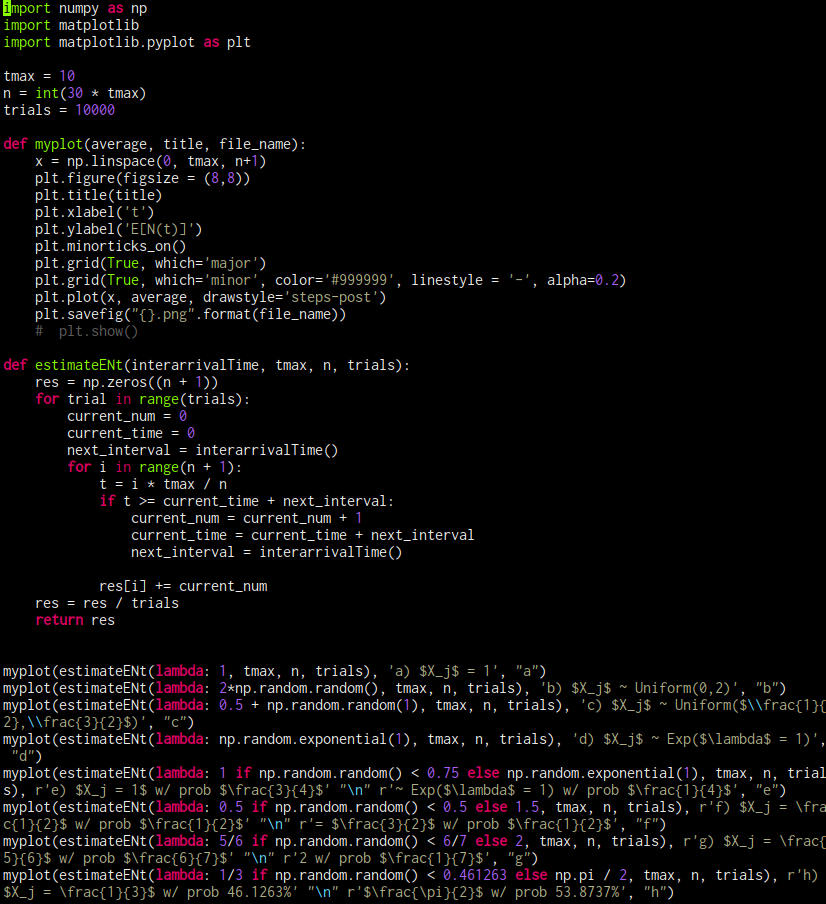
\includegraphics[width=1\linewidth]{src/code.png}
        \end{figure}
    \item Simulation Result
        \begin{figure} [t]
            \begin{subfigure}[b]{0.45\textwidth}
                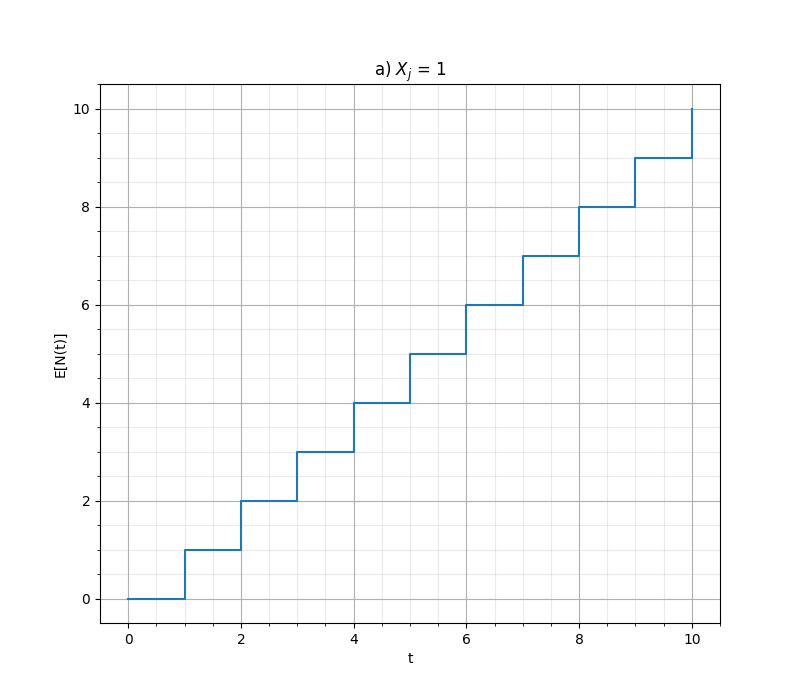
\includegraphics[width=1\linewidth]{src/a.png}
            \end{subfigure}
            \begin{subfigure}[b]{0.45\textwidth}
                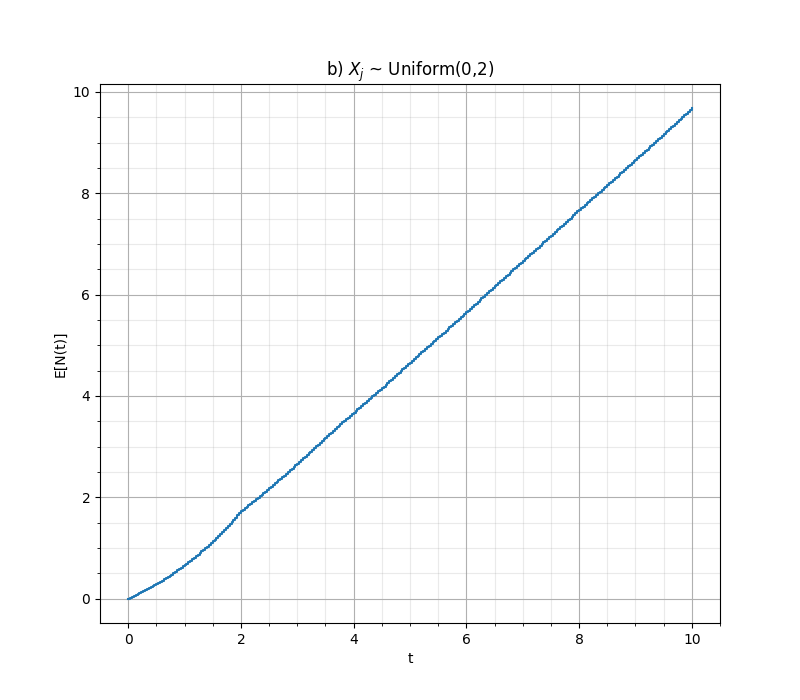
\includegraphics[width=1\linewidth]{src/b.png}
            \end{subfigure}
            \\
            \begin{subfigure}[b]{0.45\textwidth}
                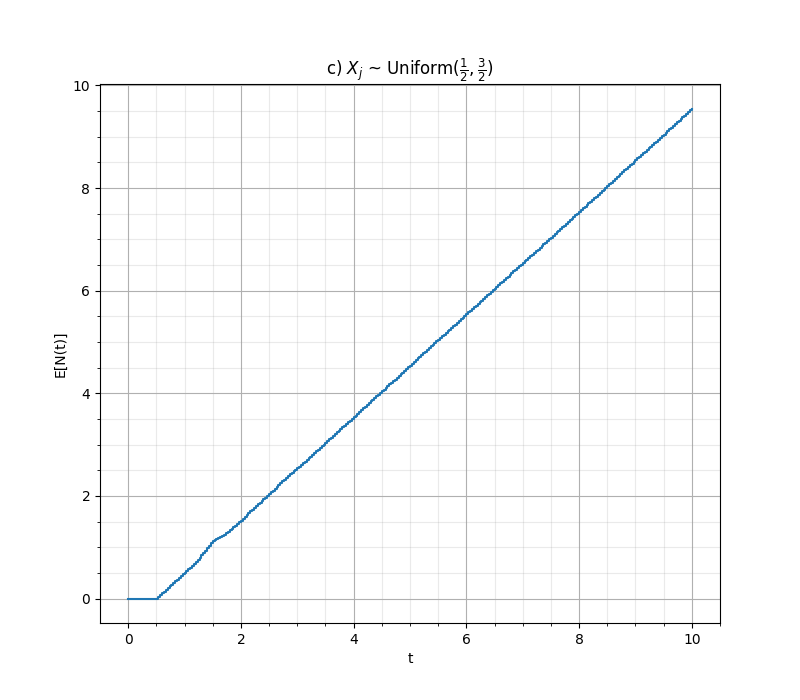
\includegraphics[width=1\linewidth]{src/c.png}
            \end{subfigure}
            \begin{subfigure}[b]{0.45\textwidth}
                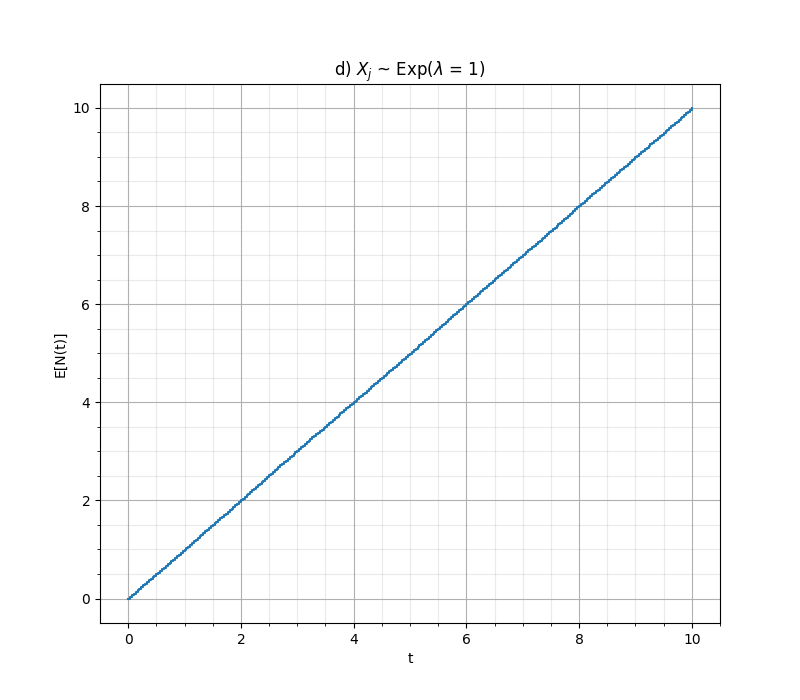
\includegraphics[width=1\linewidth]{src/d.png}
            \end{subfigure}
            \\
            \begin{subfigure}[b]{0.45\textwidth}
                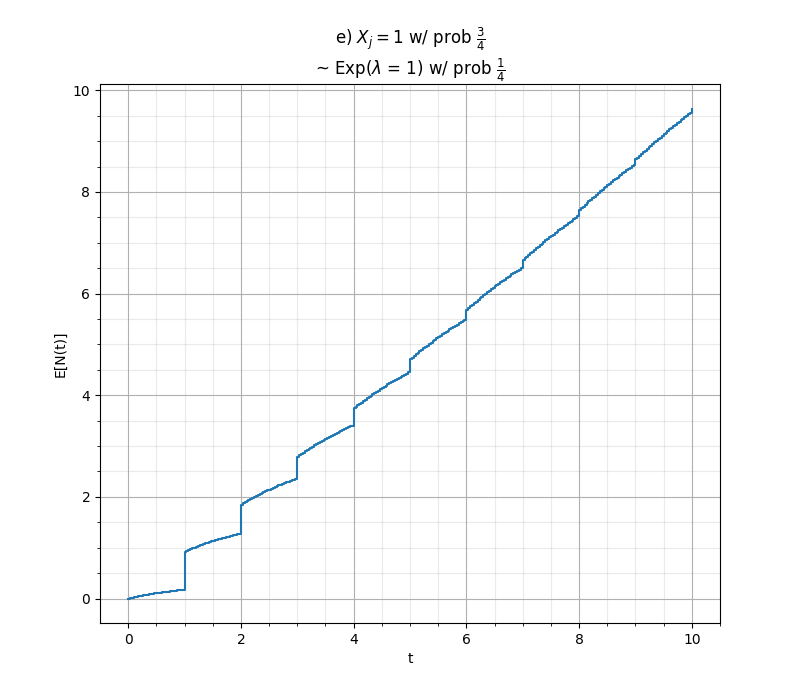
\includegraphics[width=1\linewidth]{src/e.png}
            \end{subfigure}
            \begin{subfigure}[b]{0.45\textwidth}
                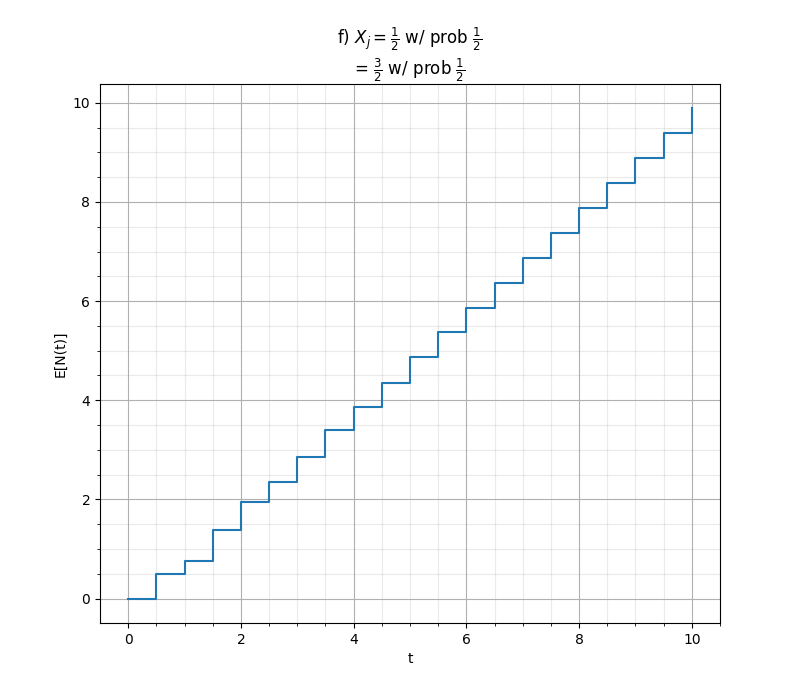
\includegraphics[width=1\linewidth]{src/f.png}
            \end{subfigure}
            \\
            \begin{subfigure}[b]{0.45\textwidth}
                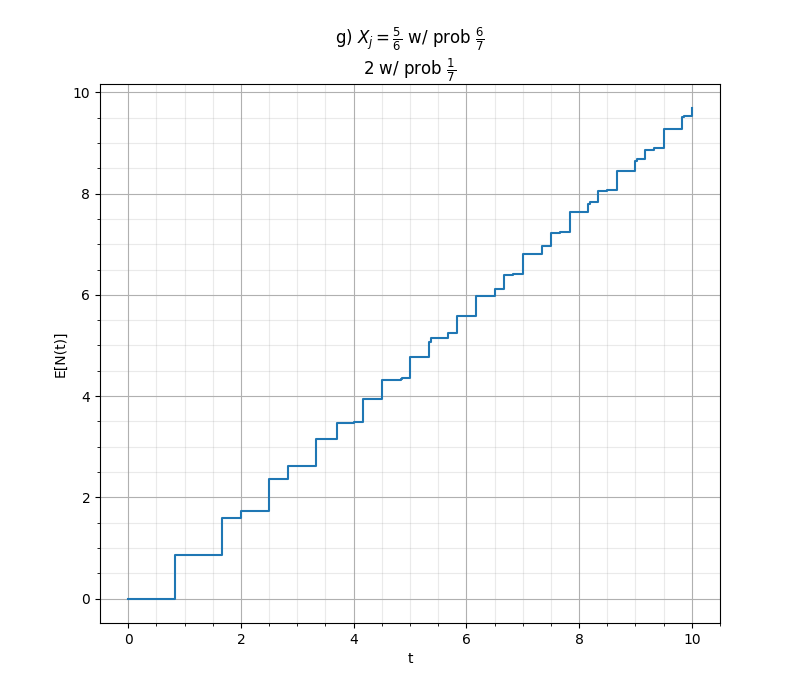
\includegraphics[width=1\linewidth]{src/g.png}
            \end{subfigure}
            \begin{subfigure}[b]{0.45\textwidth}
                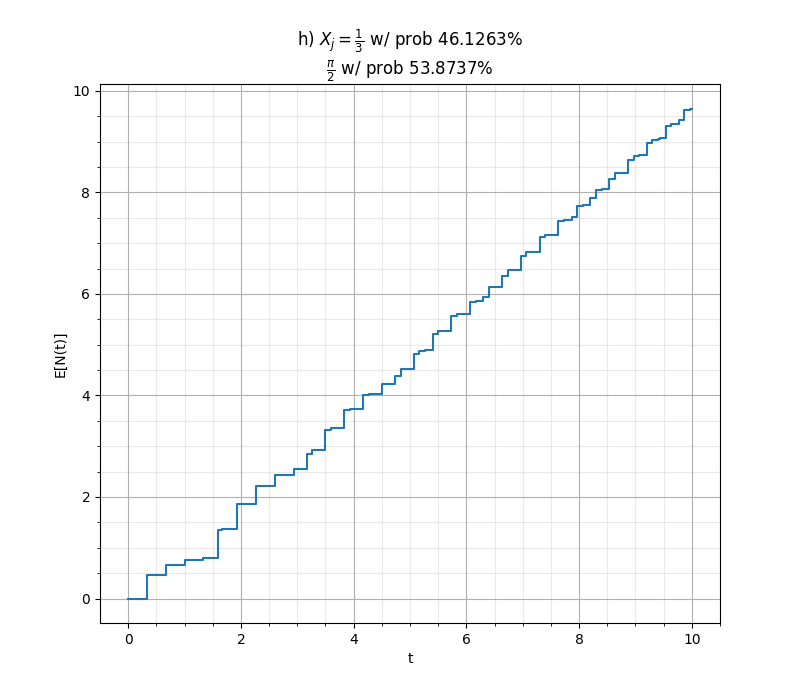
\includegraphics[width=1\linewidth]{src/h.png}
            \end{subfigure}
        \end{figure}
\end{itemize}

\end{document}
